\documentclass[10pt,letterpaper]{article}
\usepackage[top=0.85in,left=1.75in,footskip=0.75in,marginparwidth=2in]{geometry}

% use Unicode characters - try changing the option if you run into troubles with special characters (e.g. umlauts)
\usepackage[utf8]{inputenc}

% clean citations
\usepackage[noadjust]{cite}

\usepackage[shortlabels]{enumitem}
% hyperref makes references clicky. use \url{www.example.com} or \href{www.example.com}{description} to add a clicky url
\usepackage{nameref,hyperref}

% line numbers
\usepackage[right]{lineno}


% improves typesetting in LaTeX
\usepackage{microtype}
\DisableLigatures[f]{encoding = *, family = * }

% text layout - change as needed
\raggedright
\setlength{\parindent}{0.5cm}
\textwidth 5.25in 
\textheight 8.75in

% Remove % for double line spacing
%\usepackage{setspace} 
%\doublespacing

% use adjustwidth environment to exceed text width (see examples in text)
\usepackage{changepage}
\usepackage{multicol}
% adjust caption style
\usepackage[aboveskip=1pt,labelfont=bf,labelsep=period,singlelinecheck=off]{caption}

% remove brackets from references
\makeatletter
\renewcommand{\@biblabel}[1]{\quad#1.}
\makeatother

% headrule, footrule and page numbers
\usepackage{lastpage,fancyhdr,graphicx}
\usepackage{epstopdf}
\pagestyle{myheadings}
\pagestyle{fancy}
\fancyhf{}
\rfoot{\thepage/\pageref{LastPage}}
\renewcommand{\footrule}{\hrule height 2pt \vspace{2mm}}
\fancyheadoffset[L]{2.25in}
\fancyfootoffset[L]{2.25in}

% use \textcolor{color}{text} for colored text (e.g. highlight to-do areas)
\usepackage{color}

% define custom colors (this one is for figure captions)
\definecolor{Gray}{gray}{.25}

% this is required to include graphics
\usepackage{graphicx}
\usepackage{amsmath}

% use if you want to put caption to the side of the figure - see example in text
\usepackage{sidecap}

% use for have text wrap around figures
\usepackage{wrapfig}
\usepackage[pscoord]{eso-pic}
\usepackage[fulladjust]{marginnote}
\reversemarginpar

% document begins here
\begin{document}
\vspace*{0.35in}

% title goes here:
\begin{flushleft}
{\Large
\textbf\newline{Predictive learning explains emergence of objects in infants and newborn chicks}
}
\newline
% authors go here:
\\
Author 1\textsuperscript{1},
Author 2\textsuperscript{2},
Author 3\textsuperscript{1},
Author 4\textsuperscript{1},
Author 5\textsuperscript{2},
Author 6\textsuperscript{2},
Author 7\textsuperscript{1,*}
\\
\bigskip
\bf{1} Affiliation A
\\
\bf{2} Affiliation B
\\
\bigskip
* corresponding@author.mail

\end{flushleft}

\section*{Abstract}
Fitting multiple figures into very tight manuscripts while keeping it pleasant to read is challenging. Therefore figures are often simply attached to the very end of a manuscript file. While easier for the authors, this practice is inconvenient for readers. This \LaTeX template shows how to generate a compiled PDF with figures embedded into the text. It provides several examples of how to embed figures or tables directly into the text thus giving you a range of options from which you should choose the one best suited for your manuscript. Check out Schlegel et al., (2016) as example of use.

% now start line numbers
\linenumbers
% \begin{multicols}{2}
% the * after section prevents numbering
\section{Introduction}

Organizing a visual scene into structured objects and backgrounds is a crucial step towards intelligent animal behavior. The continuous stream of light rays falling on their retina creates a multitude of surfaces, all of which the brain must group into coherent objects. Remarkably, this grouping occurs despite challenges such as changes in lighting, occlusion, and perspective shifts, which can greatly obscure or alter visual information. Despite these complexities, animals achieve this rather effortlessly and almost instantaneously. Perhaps unsurprisingly, understanding this mechanism and its development has attracted considerable attention among researchers. 

One popular theory, the Gestalt processing account, posits that biological vision systems have an innate preference for ``simplicity". According to this view, objects in the world tend to exhibit simple configurations, such as smooth, continuous contours (``good continuity") and coherent motion among parts (``common fate"). Studies with developing animals have challenged the claim that such grouping principles are innately available. For instance, experiments with infants (\cite{kellman1983perception}) suggest that while they seem to exploit motion-based cues such as common fate, they fail to use static cues such as good continuity (see \ref{gestalt} for details). Other forms of synchronous but non-motion changes do not produce the same grouping effects, suggesting a privileged role for motion (\cite{jusczyk1999synchronous}). Therefore, the static grouping cues, like good continuity that adults utilize, are acquired later through development. Consistent with this interpretation, in adults with congenital blindness who had their vision restored, object parsing was initially possible only when motion cues were present \cite{ostrovsky2009visual}; only after 10-18 months of visual experience did they learn to use static cues such as good continuity. Such evidence for the primacy of motion extends beyond humans. Newly hatched chicks (\cite{wood2021one}) fail to identify and imprint on foreground objects in the absence of motion (see \ref{chicks} for details). Furthermore, neuroimaging studies in developing children show that the dorsal visual processing stream (implicated in motion processing among other tasks) matures earlier than the ventral stream (implicated in recognition of static visual cues) (\cite{ciesielski2019maturational}). Taken together, these pieces of evidence suggest that motion cues could play a foundational role in early visual development, potentially scaffolding the later acquisition of sensitivity to static grouping cues. This challenges strong innate versions of the Gestalt simplicity account and instead points toward a developmental trajectory in which perceptual organization is progressively learned.


Why and how could motion cues help? Several lines of evidence suggest that the brain continuously predicts the future state of the world (\cite{rao1999predictive, clark2013whatever, caucheteux_evidence_2023}). Such a prediction would inevitably require an understanding of motion. We propose that predictive learning underlies both the acquisition of motion cues and, eventually, the emergence of sensitivity to static cues. Lending credence to this, in both infants and chicks, when motion is made unpredictable (random video frames instead of smooth continuous motion), visual learning is impaired (\cite{kellman1984perception, wood2018development}). Specifically, we hypothesize that the ventral and dorsal streams cooperate to predict future visual inputs, thereby driving the development of motion estimation in the dorsal stream and object parsing in the ventral stream. 

To verify this, we develop a neural network model with two separate visual streams that jointly predict the next frame. When trained to minimize this next-frame prediction error on videos designed to simulate an infant's experience with moving objects, the model recapitulated their behavior -   
\begin{enumerate}[a., nolistsep]
    \item It discovered the moving objects. That is, it used the common fate cue to group into objects as a consequence of minimizing the prediction error. 
    \item It developed sensitivity to alignment; like human adults, the models eventually became sensitive to the good continuity cue. 
\end{enumerate}
When the same model was trained as a visual front-end of a model being trained to simulate chick imprinting behavior— 
\begin{enumerate}[a., nolistsep, resume]
    \item It developed background-invariant object detection that matched the behavior of biological chicks, whereas many state-of-the-art vision models failed. 
\end{enumerate}

Together, we use these results to argue that Gestalt cues are not a consequence of an innate preference for simplicity, but rather a consequence of predictive learning. Similarly, biological chicks are able to achieve background-invariant object detection not through innate knowledge of foregrounds and backgrounds but because of predictive learning as well. 



\cite{milner_how_2017}



\section{Materials and Methods}


\begin{figure}[ht] %s state preferences regarding figure placement here

% use to correct figure counter if necessary
%\renewcommand{\thefigure}{2}

\includegraphics[width=1.0\textwidth]{figs/exps_and_model2.png}

\caption{\color{Gray} \textbf{Example of a standard floating figure}. \textbf{A-F}, This figure is wrapped into the standard floating environment.}

\label{fig1} % \label works only AFTER \caption within figure environment

\end{figure}

\subsection{Gestalt processing experiments with infants. \label{gestalt}}
Infants have a well-established tendency to look longer at novel displays \cite{fantz1964visual}, which can be leveraged to probe their visual recognition. When presented with a visual stimulus, they initially fixate on it before eventually looking away (``habituation"). After this phase, when a new stimulus that is similar to or different from the habituated stimulus is presented, infants look longer at the display if they do not recognize it as the habituated stimulus  (``dishabituation") than if they recognize it as the same stimulus. Several studies (\cite{kestenbaum1987perception, kellman1983perception}) have used this to test the conditions under which infants group surfaces into objects. 

\subsubsection*{Infants discover objects through common fate but not good continuity}

To test what Gestalt cues are used for grouping, \cite{kellman1983perception} (reproduced in \cite{smith2003motion, johnson1996perception}; see \cite{valenza2006perceptual} for a reproduction in newborns) habituated 4-month-old infants to displays that contained an object center-occluded to reveal two pieces above and below. When habituated to displays where there is common motion between the two pieces, the infants grouped the two pieces into a single object, indicating that they used the Gestalt cue of common fate. Interestingly, in marked contrast to adults, they did not perceive the pieces as a single object when they were aligned but not moving. This suggests that, unlike adults, infants do not use the Gestalt cue of good continuity. In fact, adults are sensitive to such alignment cues. Changes in ``non-accidental properties" (going from aligned to non-aligned) elicit larger differences in fMRI recordings (\cite{kim2012greater}) and longer reaction times during visual searches (\cite{kubilius2017sensitivity}) compared to ``metric" changes (going from non-aligned to even more non-aligned). During development, humans go from not understanding the cue of good continuity to becoming sensitive to it. 

\subsection{Object discovery experiments with newly hatched chicks \label{chicks}}

A number of experiments seek to study the development of visual object recognition in animals, using newly hatched chicks (\textit{Gallus gallus}) as the model organism. In addition to being mobile from the first day of life, they imprint on a moving object (presumably to be near a parent) that they see during the critical period (around the first 3 days). After this critical period, they can be exposed to novel objects to see if they are identified as the imprinted object. To precisely control the visual diets of such chicks, \cite{wood2013newborn, wood2015chicken} developed specialized automated controlled-rearing chambers. These chambers have two display screens at opposite ends onto which visual stimuli can be displayed, while the remaining sides are perfectly blank. The chicks are placed in a dark chamber immediately after hatching, ensuring they are not exposed to any visual information beyond what is present in the chamber. During the training phase, the chicks are exposed to a visual stimulus displayed on either of the two screens to which they are expected to imprint. After the conclusion of this phase, for testing, one of these screens displays the imprinted stimulus while the other displays a novel distractor stimulus. The chicks spend more time near the stimulus they recognize as the imprinted stimulus, while staying away from the distractor. 

\subsubsection*{Newly hatched chicks discover objects during imprinting}
To test chicks' abilities in object discovery, \cite{wood2021one} imprinted them on displays that contained a foreground object that has rotational movement on a static natural background. They were then tested with conditions where the familiar foreground object was placed on novel backgrounds while the other display contained novel distractor objects on the familiar background. In these conditions, the chicks spent more time near the familiar foreground object indicating that they had parsed the foreground and background in these displays. Another set of chicks that were imprinted on similar displays but with no foreground movement showed impaired foreground detection ability suggesting again that the motion cues were necessary. 

When DNNs are trained on an exact replica of the rearing chamber created using computer graphics, they failed to detect objects in this way (\cite{garimella2024newborn}). A slew of DNNs were trained using reinforcement learning to maximize an imprinting reward (rewarded to be near the foreground object). When these DNNs were tested on the foreground-background swap conditions like the chicks, they failed to generalize to detecting the imprinted object indicating that the DNNs failed at background-invariant object detection. 

\subsection*{A two stream model of vision}

The two-streams hypothesis (\cite{goodale1992separate}) posits that visual information is processed by two distinct pathways, the ventral stream (``what" pathway) and the dorsal stream (``how/where" pathway). The visual stimuli that fall on the retina pass through the LGN and V1 where it splits into the two streams. We model the retina and LGN using a deep neural network ($ \phi_{\theta e}$) that when applied to two temporally consecutive visual stimuli $x_t$ and $x_{t+1}$ produces -

\[ y_t = \phi_{\theta e}(x_t) \quad y_{t+1} = \phi_{\theta e}(x_{t+1}) \]

A subset of the neurons in V1 pass the visual signal into the higher layers of the ventral stream. The subsequent stages (V2, V4, IT) in this stream process the visual information to recognize objects by extracting static cues such as shape, orientation, color, and texture. These cues are utilized to group locations in the visual field into coherent regions, for example, the foreground and the background. We model this using a 3-layer deep convolutional neural network ($ \phi_{\theta v}$) followed by the softmax function which for every spatial location predicts the probability of it being in the foreground rather than the background -

\[ f_v = softmax(\phi_{\theta v}(y_t)) \]

The direction-selective neurons in the V1 innervate into the dorsal stream. MT and MST areas within the dorsal stream are tasked with detecting and processing object motion. Our model of the dorsal stream ($ \phi_{\theta d} $) consisting of a 3-layer 3D convolutional neural network takes in the features of the two consecutive visual stimuli ($y_t$ and $y_{t+1}$) to detect the motion between them - 

\[ f_d = \phi_{\theta d}(y_t, y_{t+1}) \]

The static features $f_v$ (estimate of what is expected to move in the frame) and motion features $f_d$ (estimate of what has moved in the two frames) are then combined and used along with the current frame $x_t$ to predict the future frame. 
\begin{align*}
&h = f_v \circ f_d \\
&\hat{x}_{t+1} = predictor(x_t, h)
\end{align*}

This predicted frame can now be compared to the ground truth frame to calculate a prediction error $e$ using a metric $d$. We choose a simple $L^2$ distance as our metric. All the components of our model can be trained using gradient descent to minimize this prediction error. 

\[ e = d(\hat{x}_{t+1}, x_{t+1}) \]


\section*{Results}

\begin{figure}[ht] %s state preferences regarding figure placement here

% use to correct figure counter if necessary
%\renewcommand{\thefigure}{2}


\includegraphics[width=1.0\textwidth]{figs/miou.png}

\caption{\color{Gray} \textbf{Example of a standard floating figure}. \textbf{A-F}, This figure is wrapped into the standard floating environment.}

\label{figmiou} % \label works only AFTER \caption within figure environment

\end{figure}

\subsection*{Predictive learning begets common fate.}

To train the model, we created a new dataset containing objects in motion. We generate 2500 videos (each 20 frames long) where a foreground object (a rectangle) of random color and texture moves over the background consisting of random shapes. The only signal identifying it as a coherent single object was the common motion of its pixels and the only static cue to identify it was its shape. We train our model to minimize the next frame prediction error on these videos. As the model is training, we compare its estimate of the object ($f_v$) and compare it to the ground truth object segmentation masks (fig). 


\subsection*{Predictive learning begets good continuity.}

\begin{figure}[ht] %s state preferences regarding figure placement here

% use to correct figure counter if necessary
%\renewcommand{\thefigure}{2}

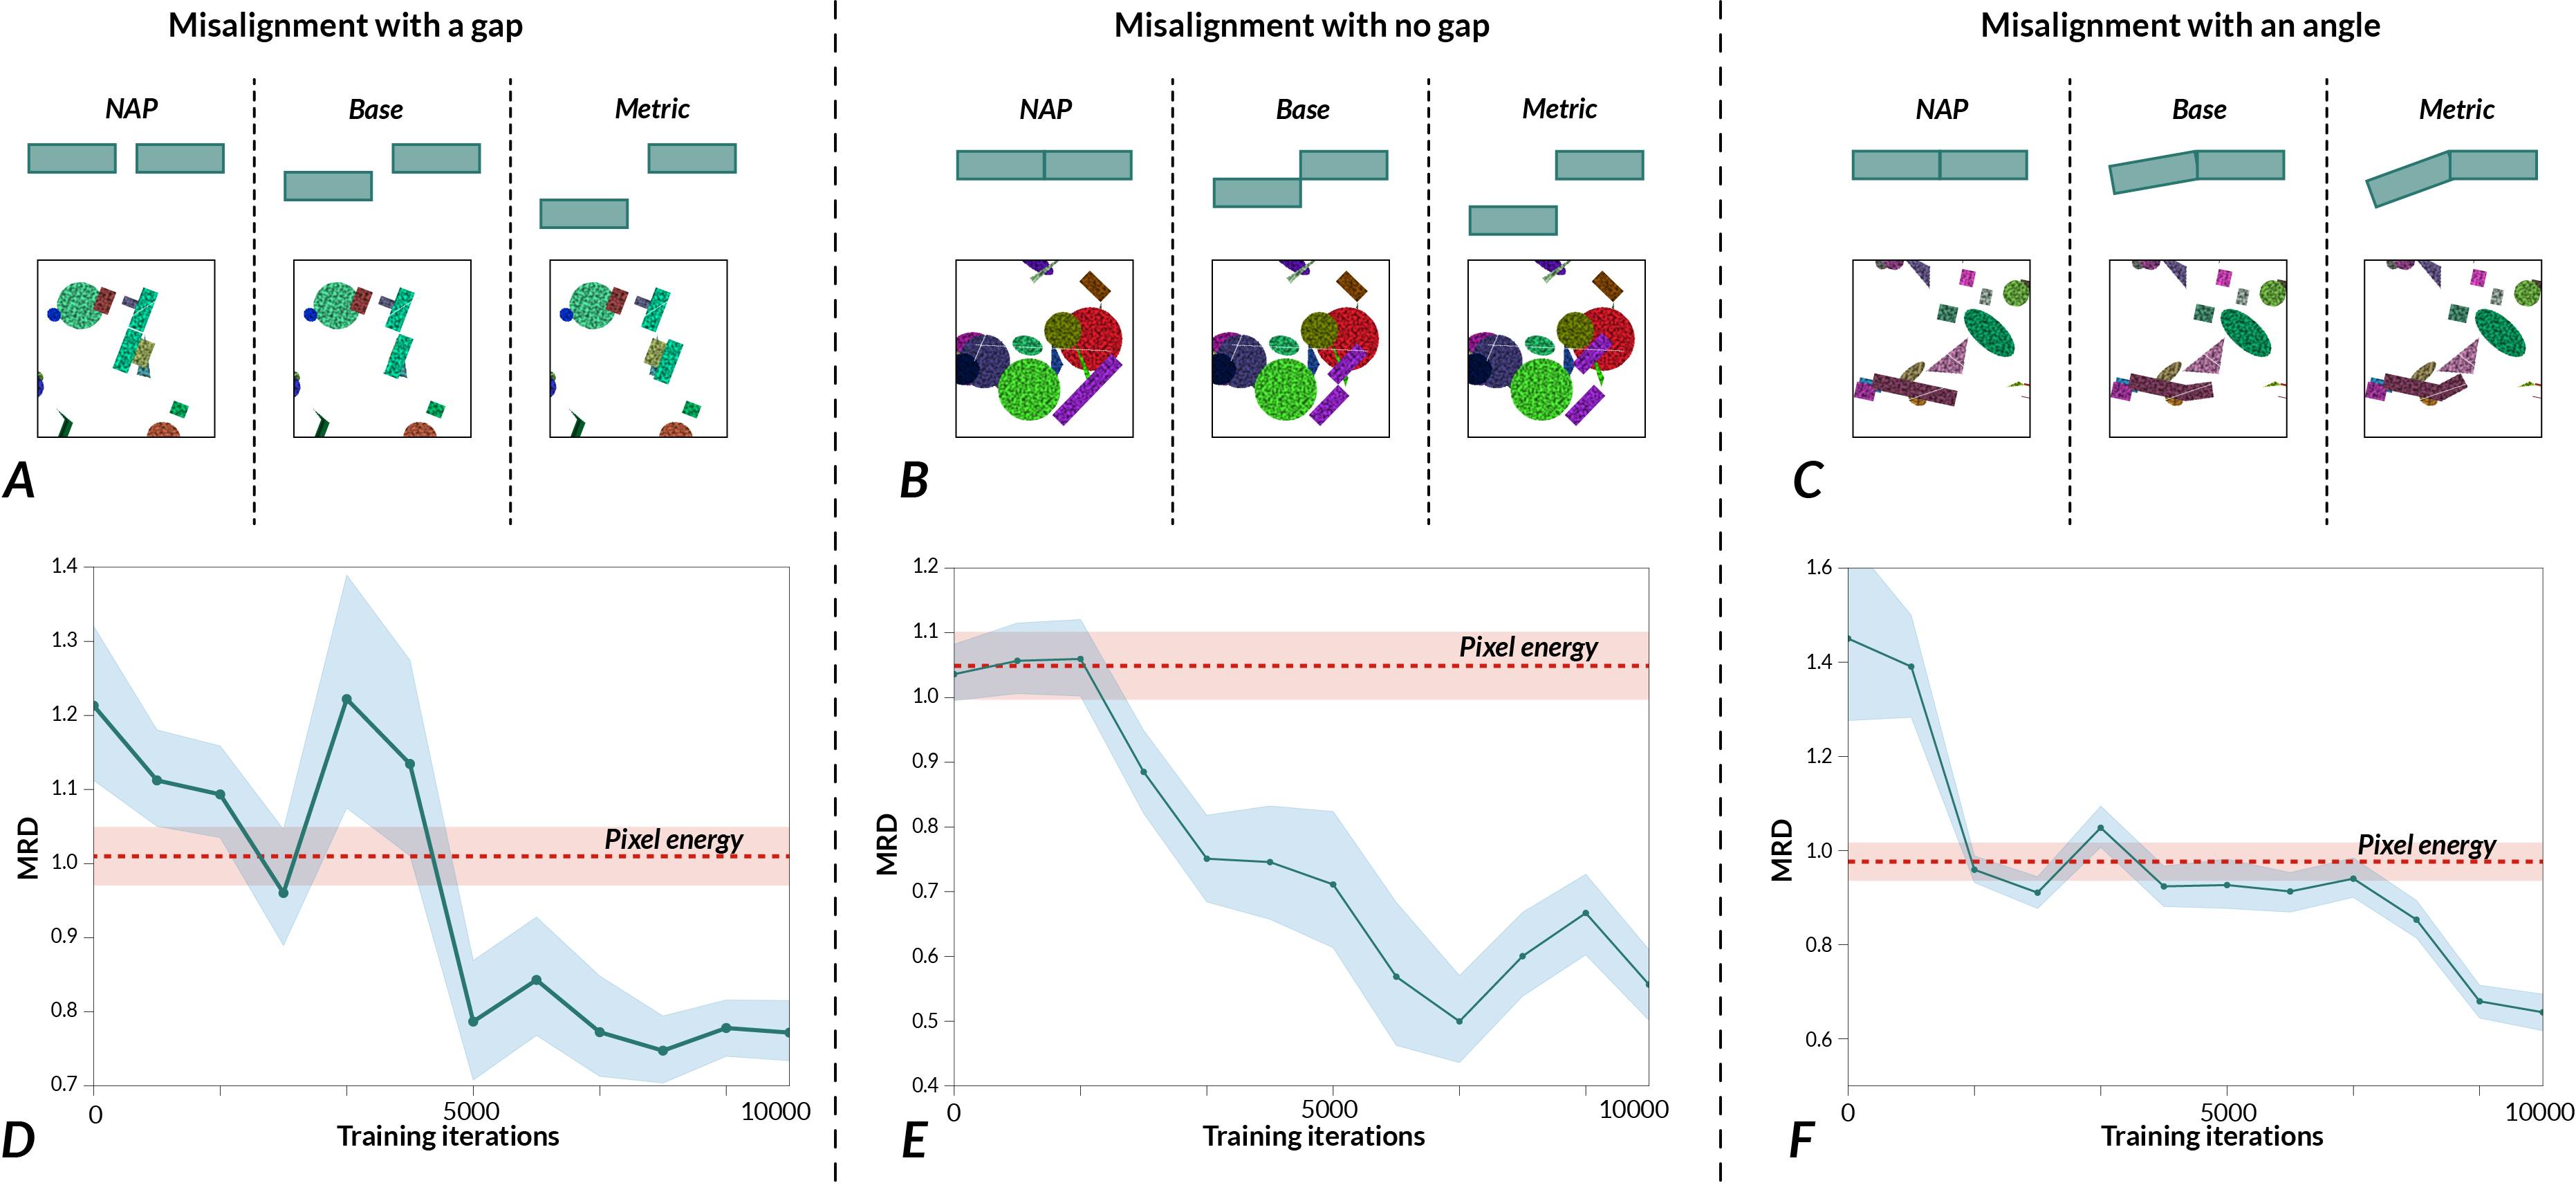
\includegraphics[width=\textwidth]{figs/mrd.png}

\caption{\color{Gray} \textbf{Example of a standard floating figure}. \textbf{A-F}, This figure is wrapped into the standard floating environment.}

\label{figmrd} % \label works only AFTER \caption within figure environment

\end{figure}

To test human subjects' sensitivity to alignment cues, \cite{kim2012greater} created triplets of stimuli - non-accidental property (NAP) condition (edges are aligned), base condition (edges are misaligned by some amount $m$) and metric condition (edges are misaligned by amount $2\times m$). These triplets are created such that in pixel space the difference between NAP stimuli and base stimuli is the same as the difference between base stimuli and metric stimuli. That is, the mean relative dissimilarity (MRD) is close to 1 - 

\[ MRD_{pixel} = \frac{1}{N} \sum_{i=1}^{N} \frac{d(x_i^{base}, x_i^{metric})}{d(x_i^{base}, x_i^{NAP}) } \approx 1\]

Despite this, when the subjects are presented these stimuli their lateral occipital cortex (implicated in recognition of object shape) indicated greater sensitivity for NAP to base pair than base to metric pair (\cite{kim2012greater}). If our model developed such sensitivity, MRD calculated using its ventral stream features should be well below 1. To test this, we created similar triplets across three variants (fig). 

\[ MRD_{model} = \frac{1}{N} \sum_{i=1}^{N} \frac{d(\phi_{\theta v}(x_i^{base}), \phi_{\theta v}(x_i^{metric}))}{d(\phi_{\theta v}(x_i^{base}), \phi_{\theta v}(x_i^{NAP})) }\]

\subsection*{Same model explains object parsing in newborn chicks.}

We then use the same model as a front-end vision module of the artificial chick. When the model is trained on sequence of frames as the artificial chick learns to navigate (imprint), it learns background-invariant recognition, unlike the off-the-shelf CNNs. 

\begin{figure}[ht] 

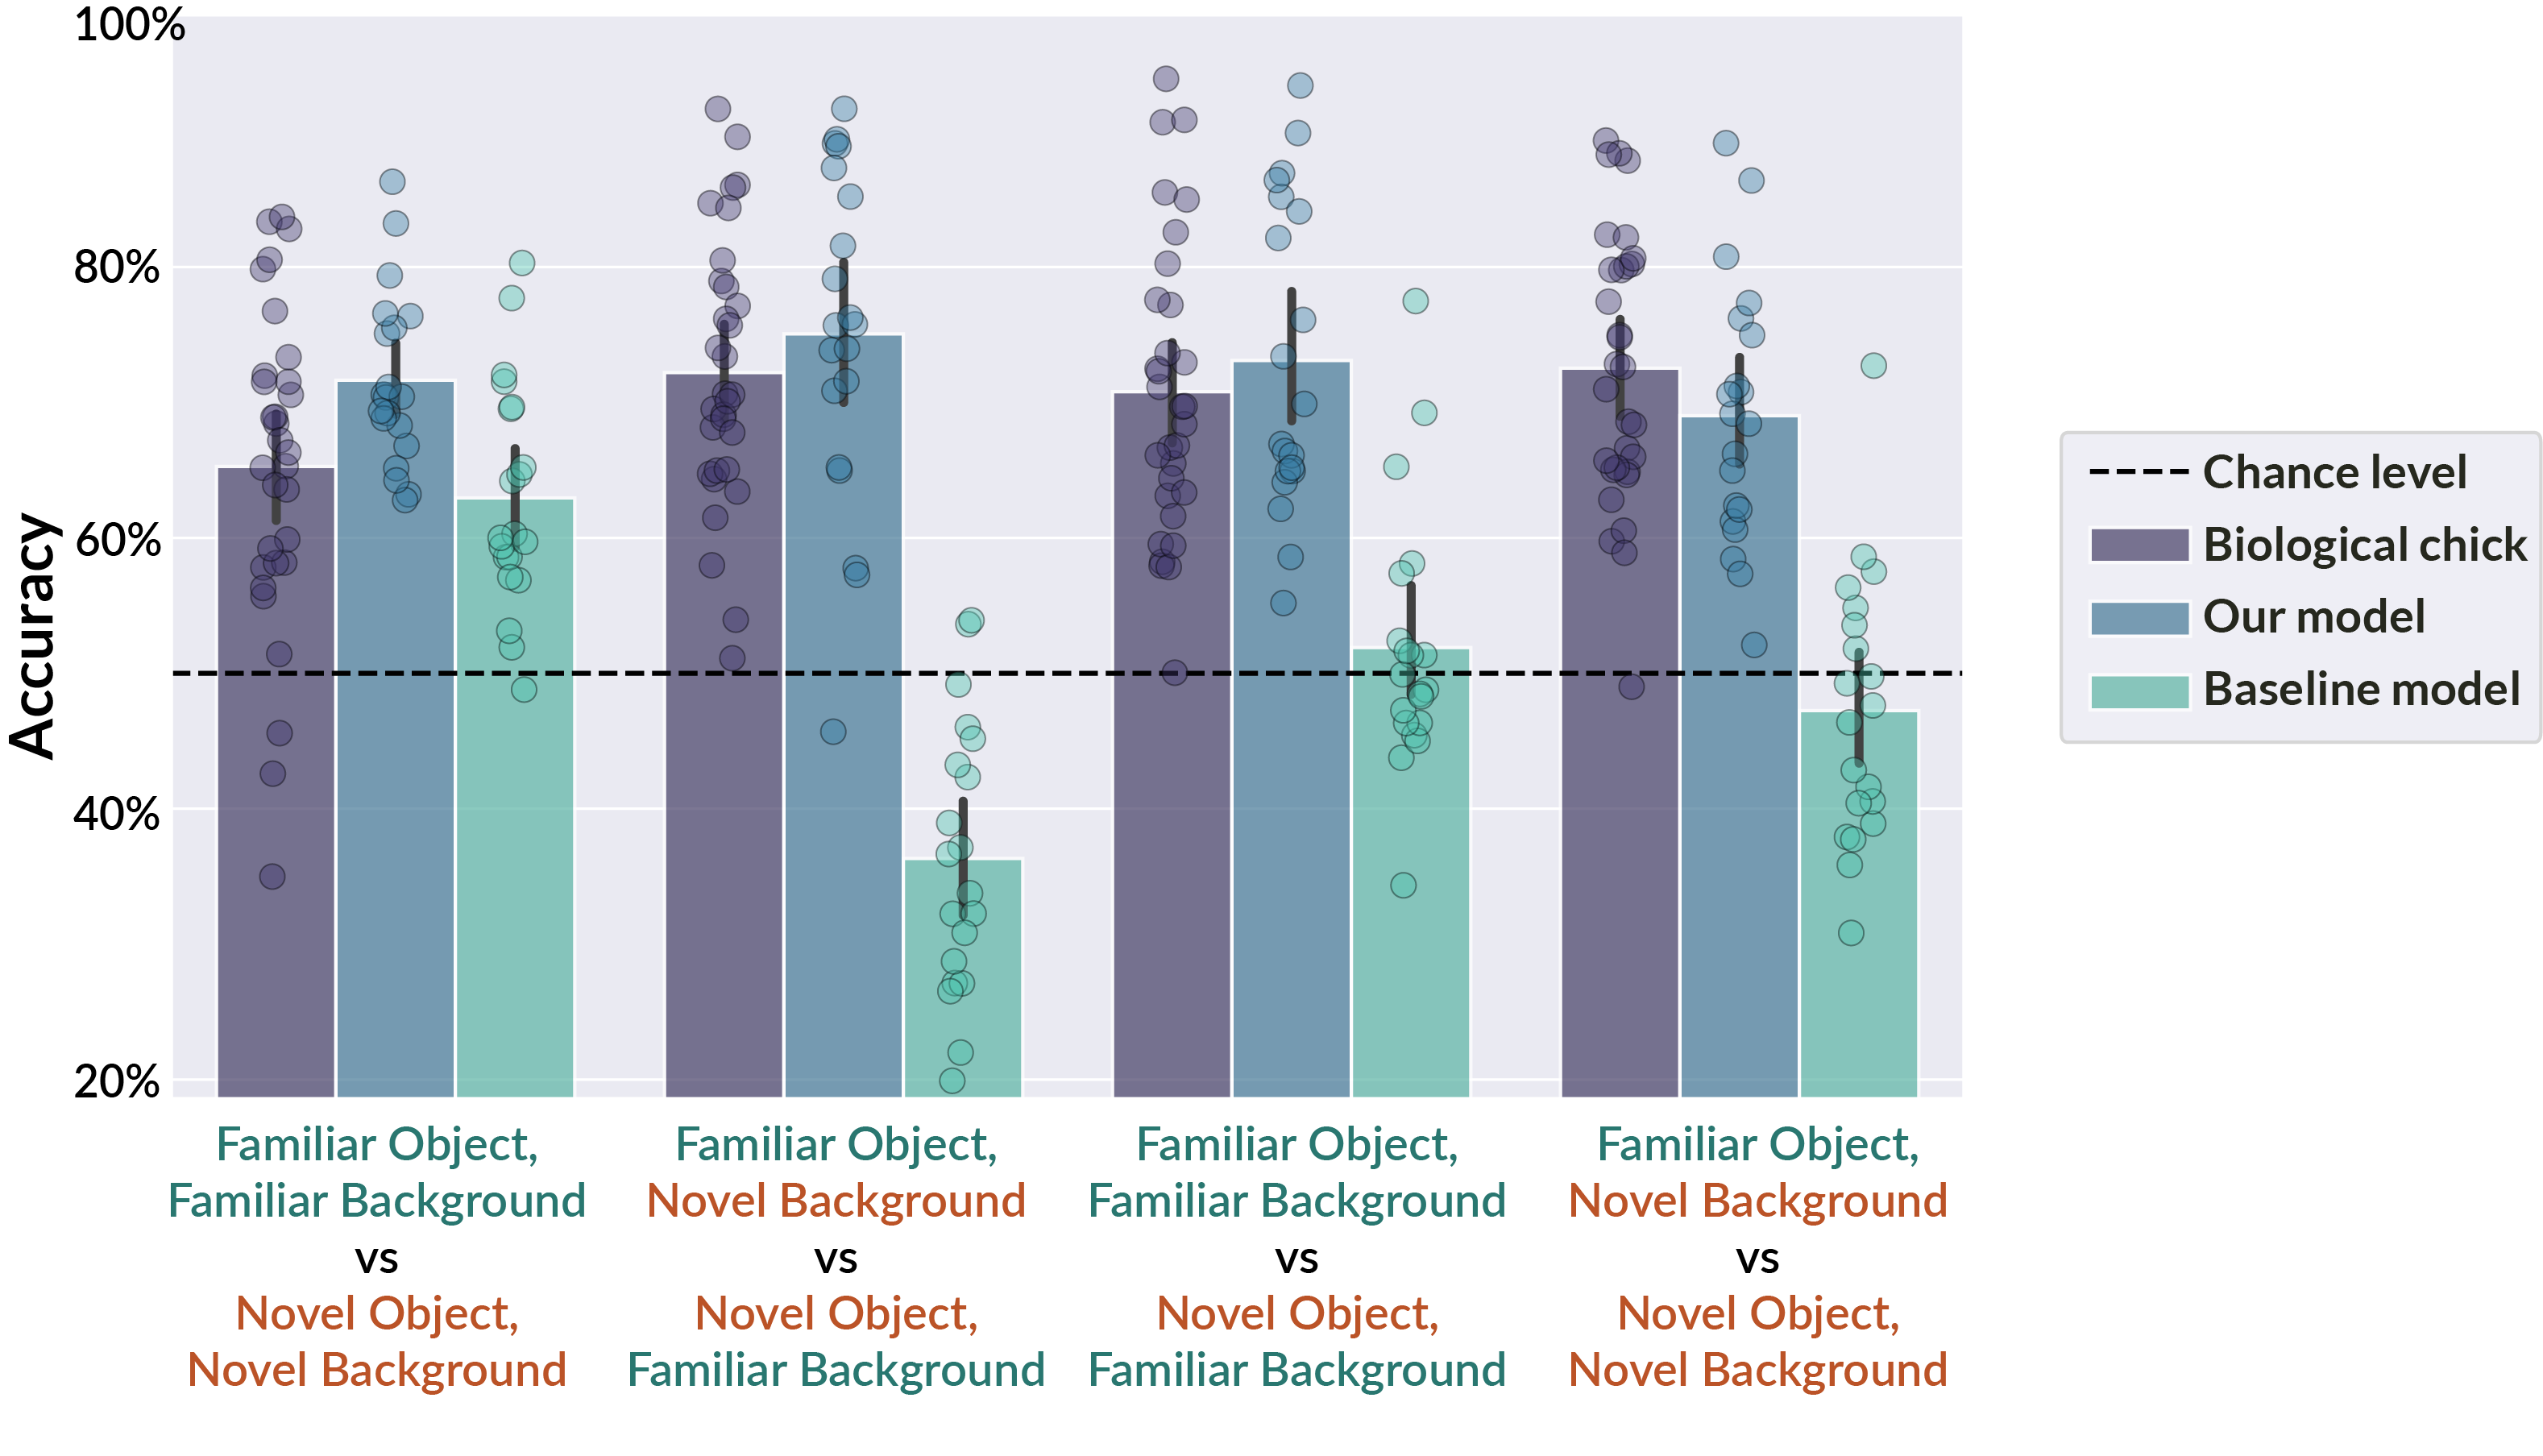
\includegraphics[width=\textwidth]{figs/rl_chick.png}

\caption{\color{Gray} \textbf{Example of a standard floating figure}. \textbf{A-F}, This figure is wrapped into the standard floating environment.}

\label{figmrd} % \label works only AFTER \caption within figure environment

\end{figure}


%\clearpage makes sure that all above content is printed at this point and does not invade into the upcoming content
%\clearpage

\section*{Discussion}
\subsection*{Subsection heading.}

Lorem ipsum dolor sit amet, consectetur adipiscing elit. Aliquam bibendum finibus diam, gravida sagittis lorem gravida vitae. Interdum et malesuada fames ac ante ipsum primis in faucibus. Nulla in diam tristique ante posuere tristique. Donec interdum purus sit amet nisl accumsan consectetur. Fusce aliquet libero mi, quis ornare dolor congue ullamcorper. Nulla nulla urna, molestie in urna sed, lacinia volutpat eros. Ut mi libero, elementum scelerisque ipsum vel, hendrerit fermentum turpis. Aliquam sit amet leo sodales, egestas augue id, fermentum nulla. Aenean vel cursus ante, et pellentesque eros. Nulla ac neque nec justo posuere commodo sit amet sit amet justo. Aliquam tincidunt tempor ex nec tincidunt. In ullamcorper vehicula lobortis. 

%\clearpage

\section*{Supporting Information}
If you intend to keep supporting files separately you can do so and just provide figure captions here. Optionally make clicky links to the online file using \verb!\href{url}{description}!.

%These commands reset the figure counter and add "S" to the figure caption (e.g. "Figure S1"). This is in case you want to add actual figures and not just captions.
\setcounter{figure}{0}
\renewcommand{\thefigure}{S\arabic{figure}}

% You can use the \nameref{label} command to cite supporting items in the text.
\subsection*{S1 Figure}
\label{example_label}
{\bf Caption of Figure S1.} \textbf{A}, If you want to reference supporting figures in the text, use the \verb!\nameref{}!. command. This will reference the section's heading: \nameref{example_label}.

\subsection*{S2 Video}
\label{example_video}
{\bf Example Video.} Use \href{www.youtube.com}{clicky links} to the online sources of the files.

%\clearpage

\section*{Acknowledgments}
We thank just about everybody.

\nolinenumbers

% \end{multicols}
%This is where your bibliography is generated. Make sure that your .bib file is actually called library.bib
\bibliography{library}

%This defines the bibliographies style. Search online for a list of available styles.
\bibliographystyle{abbrv}

\end{document}

